\documentclass[11pt,a4paper,twoside]{article}
\usepackage[dutch]{babel}
%laad de pakketten nodig om wiskunde weer te geven :
\usepackage{amsmath,amssymb,amsfonts,textcomp}
%laad de pakketten voor figuren :
\usepackage{graphicx}
\usepackage{float,flafter}
\usepackage{hyperref}
\usepackage{inputenc}
%zet de bladspiegel :
\setlength\paperwidth{20.999cm}\setlength\paperheight{29.699cm}\setlength\voffset{-1in}\setlength\hoffset{-1in}\setlength\topmargin{1.499cm}\setlength\headheight{12pt}\setlength\headsep{0cm}\setlength\footskip{1.131cm}\setlength\textheight{25cm}\setlength\oddsidemargin{2.499cm}\setlength\textwidth{16.5cm}

\begin{document}
\begin{center}
\hrule

\vspace{.4cm}
{\bf {\Huge EEE220 Lab Report 1}}
\vspace{.2cm}
\end{center}
{\bf Name:\ Wang Lu }  \\
{\bf ID Number:\ 1301383} \hspace{\fill} 28 March 2016 \\
\hrule


\section{Experiment 1}
This section aims at determining the sensitivity of a Wheatstone bridge arrangement and compare with theoretical expression for the sensitivity. The circuit is shown as below. 

\begin{figure}[!h]
\centering
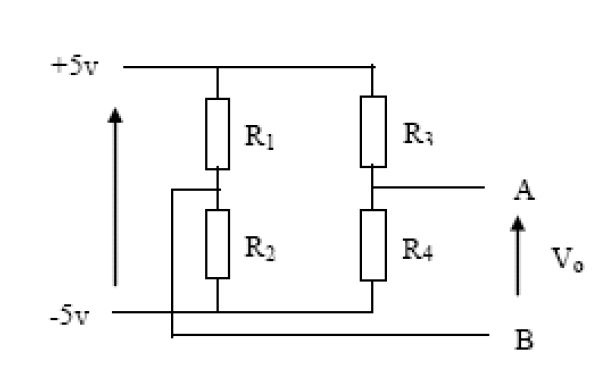
\includegraphics[width=0.6\linewidth]{1}
\caption{Wheatstone bridge}
\label{f1}
\end{figure}

\subsection{Results}

\begin{table}[!h]
\centering
\begin{tabular}{|c|c|c|c|}
	\hline
	$\delta R $ & $\delta R/R \ (10^{-3})$ \  & $ \delta V $(mV) & Theoretical $\delta$ V (mV) \\
	\hline\hline
	0 & 0.00 & 0.05 & 0.00\\
	\hline
	1 & 8.33 & 20.00 &20.83\\
	\hline
	2 & 16.67 & 40.90 &41.67\\
	\hline
	3 & 25.00 & 61.40 &62.50\\
	\hline
	4 & 33.33 & 81.90 &83.33\\
	\hline
	5 & 41.67 & 102.00 &104.17\\
	\hline
	6 & 50.00 & 122.30 &125.00\\
	\hline
	7 & 58.33 & 142.00 &145.83\\
	\hline
	8 & 66.67 & 161.70 &166.67\\
	\hline
	9 & 75.00 & 181.50 &187.50\\
	\hline
\end{tabular}
\caption{Measurement result of Exp.1}
\label{t1}
\end{table}



\begin{figure}[!h]
	\centering
	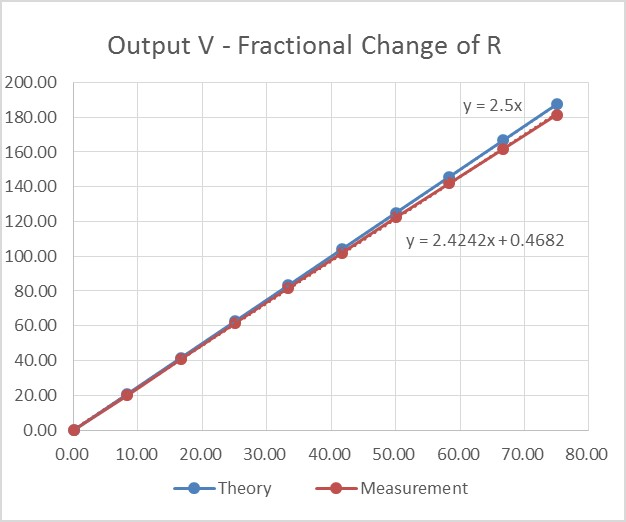
\includegraphics[width=0.62\linewidth]{2}
	\caption{Plot of output against fractional change in resistance}
	\label{f2}
\end{figure}

\subsection{Answsers to Questions}
\begin{enumerate}
	\item 
\textbf{	Experimental Sensitivity = 2.4242} \\
	The line equation can be seen in Figure\ref{f2} is \\
	\begin{equation}
	  \delta V = 2.4242\ \frac{\delta R}{R} + 0.4682
	\end{equation}
	
	\item
\textbf{	Theoretical Sensitivity = 2.5} \\
	According to the equation in the instrustion, the output voltage has the relationship with arm resistors as below. 
		\begin{equation}
		\delta V = \frac{ER_{4}}{R_{3}+R_{4}+\delta R} - \frac{ER_{4}}{R_{3}+R_{4}}
		\end{equation}
	By selecting $R_{1}=R_{2}$ and with $R_{4}$ set equal to the gauge resistance, the output voltage can be expressed as below. The coefficient of the equation is its sensitivity. 
		\begin{equation}
		|\delta V |=\left[ \frac{E}{4}\right] \ \frac{\delta R}{R}, \ \ where\ E=10\ V, k=2.5
		\end{equation}
		
	\item
\textbf{	Comments}\\
	It can be seen that the output voltage and fractional change of the resistor have the linear relationship, which fits the characteristic of the Wheatstone bridge configuration.Therefore, we could measure the small change of the resistance via the measurement of the fractional change in voltage in the following experiments.The experimental results are quite close to the theoretical one. The output voltage is zero when there is no strain. However, the initial condition cannot reach perfect in practical, and the slight deviation comes from the accuracy of measurement, along with the influence of the temperature. 
\end{enumerate}
\pagebreak

\section{Experiment 2}
This section aims at investigating the relative sensitivity of a single active gauge bridge, and verify the function of temperature compensation.The circuit is shown as below. 

\begin{figure}[!h]
	\centering
	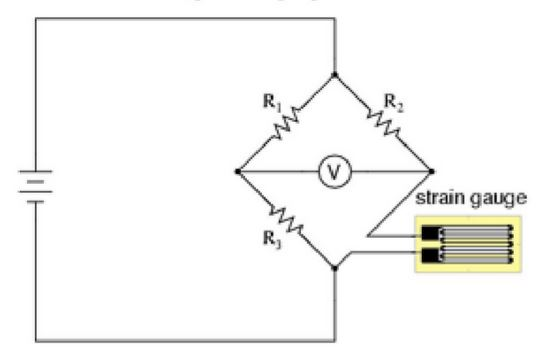
\includegraphics[width=0.5\linewidth]{3}
	\caption{Wheatstone bridge with single gauge}
	\label{f3}
\end{figure}

\subsection{Results}

\begin{table}[!h]
	\centering
	\begin{tabular}{|c|c|c|c|c|}
		\hline
		Mass (kg) & $\delta V \ (mV)$ & $y\ (mV)$ & $\ \varepsilon \ 10^{-3} \ $ & $ G \ \ $  \\
		\hline\hline
		0.0 & 0.01 & 0 & 0.0000 & NA\\
		\hline
		0.5 & 0.29 & 0.095 &0.0596 & 1.9475\\
		\hline
		1.0 & 0.58 & 0.184 &0.1154 &2.0110\\
		\hline
		1.5 & 0.85 & 0.273 &0.1712 &1.9863\\
		\hline
		2.0 & 1.12 & 0.361 &0.2263 &1.9793\\
		\hline
		2.5 & 1.40 & 0.450 &0.2822 &1.9848\\
		\hline
		3.0 & 1.68 & 0.540 &0.3386 &1.9848\\
		\hline
	
	\end{tabular}
	\caption{Measurement result of Exp.2}
	\label{t2}
\end{table}

\subsection{Answsers to Questions}
\begin{enumerate}
\item
\textbf{Use the temperautre compensation stain gauge to reduce its influence.}\\
In the experiment, it is required that the change of strain is directly reflected by the change of resistance. However, the temperature will also influence the stain gauge material, and the specimen material. Strain gauges that are not self-temperature-compensated, which can be temperature compensated by use of the dummy gauge technique. However, this procedure cannot totally remove the effect.

\item 
\textbf{There is no variation in temperature.} \\
with installed with an identical dummy gauge on the unstrained sample,the sample with dummy gauge is in thermal contact with the test specimen, which is near the active gauge. Moreover, the dummy gauge is also connected into the bridge, which is adjacent to the active one.Therefore, the temperature influence on the dummy and active gauges will cancel each other.\\

The process can also be verified mathematically.Let the fractional change in the resistance of the active gauge due to strain be $x$ and the change dut to the temperature effects be $y$. Therefore, $R_{3}$ and  $R_{4}$ would be 
		\begin{equation}
		R_{g}=R_{3}(1+x)(1+y) 
		\end{equation}
		\begin{equation}
		R_{g}^{'}=R_{3}(1+y) 
		\end{equation}
		
The output signal $\delta V $, with  $R_{1}$ and  $R_{2}$ fixed at $R_{3}$ follows
	\begin{equation}
	\delta V = E \left[\frac{R_{3}(1+x)(1+y)}{R_{3}(1+x)(1+y)+R_{3}(1+y) }- \frac{1}{2} \right ]=\frac{EX}{2(2+X)}
	\end{equation}
Therefore, it can be seen that the effect of temperature does not qppear in the bridge output. 
\end{enumerate}

\section{Experiment 3}
This section aims at investigating the relative sensitivity of a single and a double-active gauge bridge, and determine the gauge factor G.The circuit is shown as below. 

\begin{figure}[!h]
	\centering
	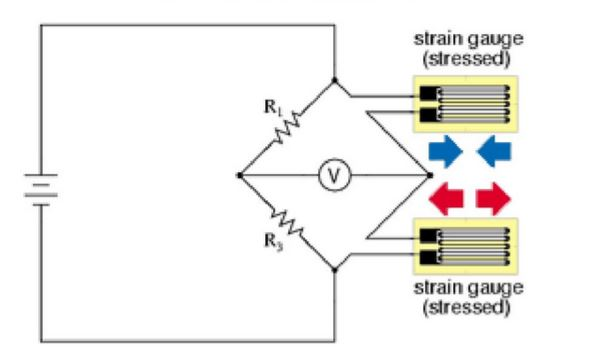
\includegraphics[width=0.5\linewidth]{4}
	\caption{Wheatstone bridge with double gauge}
	\label{f4}
\end{figure}

\subsection{Results}

\begin{table}[!h]
	\centering
	\begin{tabular}{|c|c|c|c|c|}
		\hline
		Mass (kg) & $\delta V \ (mV)$ & $y\ (mV)$ & $\ \varepsilon \ 10^{-3} \ $ & $ G \ \ $  \\
		\hline\hline
		0.0 & 0.048 & 0.000 &0.0000 & NA\\
		\hline
		0.5 & 0.506 & 0.073 &0.0458 &2.2110\\
		\hline
		1.0 & 0.060 & 0.162 &0.1016 &2.0871\\
		\hline
		1.5 & 0.580 & 0.251 &0.1574 &2.0079\\
		\hline
		2.0 & 2.110 & 0.341 &0.2138 &1.9737\\
		\hline
		2.5 & 2.620 & 0.429 &0.2690 &1.9481\\
		\hline
		3.0 & 3.130 & 0.519 &0.3254 &1.9237\\
		\hline
		
	\end{tabular}
	\caption{Measurement result of Exp.3}
	\label{t3}
\end{table}
\pagebreak

\begin{figure}[!h]
	\centering
	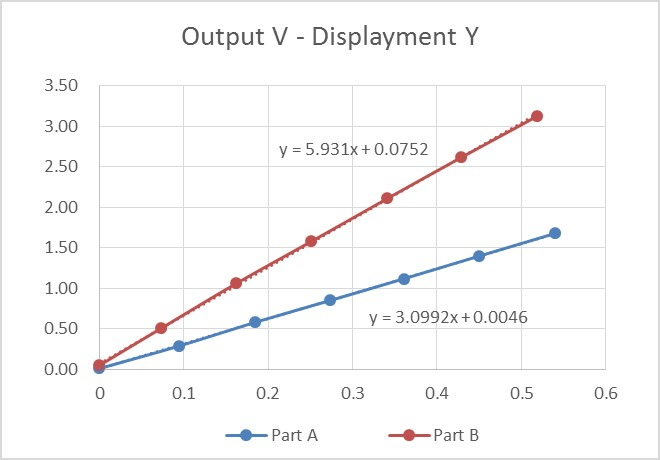
\includegraphics[width=0.7\linewidth]{5}
	\caption{Output and the displayment in Exp.3 and Exp.4}
	\label{f5}
\end{figure}

\subsection{Answsers to Questions}
\begin{enumerate}
\item
\textbf{The coefficient of the line equation in Exp.4 is twice of that in Exp.3.} \\
It can be seen that the output voltage is proportion to the displacement, no matter the single or double-active gauges. The relationship in single gauge with temperature compensation experiment is 

	\begin{equation}
	\delta V = 3.099y + 0.0046
	\end{equation}
The relationship in double-gauge experiment is  

	\begin{equation}
	\delta V = 5.931y + 0.0752
	\end{equation}
The slop indicates its sensitivity, while in theory, the sensitivity of the bridge to strain can be doubled by making both gauges active in a half-bridge configuration. Therefore, in practical, the ratio of two coefficients is 
	\begin{equation}
	\frac{k_{2}}{k_{1}}= \frac{5.931}{3.099} \approx 2
	\end{equation}

\item
\textbf{The strain ($\varepsilon$) and the gauge factor ($G$) is calculated in Table\ref{t2} and Table\ref{t3}.}\\
The calculation in where $Mass=0.5kg$, single-gauge, will be taken as an example. \\
According to the Equation in Lab Mannual, the strain can be calculated as below.
	\begin{equation}
	\varepsilon = \frac{4hy}{l^{2}}
	\end{equation}
According to the parameters of the equipment,where $h=6.27mm, l=200mm$, and when $Mass=0.5kg, y=0.095mm$, the strain can be calculated as below. 
    \begin{equation*}
    \varepsilon = \frac{4 \times 6.27 \times 0.095}{200^{2}}=0.0596 \times 10^{-3}
    \end{equation*}
According to the Equation 
	\begin{equation}
	Output voltage = Sensitivity \cdot Gauge Factor \cdot Strain
	\end{equation}
The Gauge Factor can be calculated where $ \varepsilon =0.0596 \times 10^{-3},	\delta V =0.29 mV,  Sensitivity= 2.5$
	\begin{equation*}
	G = \frac{0.29}{0.0596\times 2.5}=1.9475\approx\textbf{ 2}
	\end{equation*}
The experimental value of gauge factor is approximate to its theoretical value. 

\item
\textbf{The sensitivity of strain gauge is increased using mutiple strain gauges.}\\
\begin{figure}[!h]
	\centering
	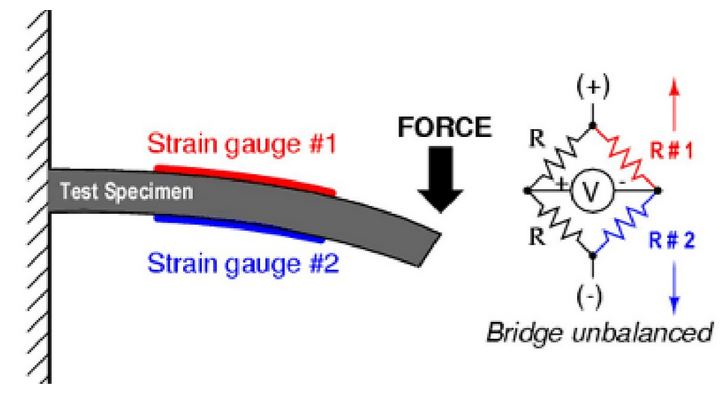
\includegraphics[width=0.6\linewidth]{6}
	\caption{Doule stain gauge with force}
	\label{f6}
\end{figure}

In the experiment, when using double-gauge, the sensitivity is doubled. From the picture, it can be seen that when two identical gauges are attached to the test specimen, the tensile strain improsed on the gauge is equal to the compressive strain. Both gauges will change in resistance by the same amount, but one increase while the other decrease. It causes the double of sensitivity. It can be further increased by making all four resistances of the arms of the bridge by active strain gauges, which is called full-bridge strain gauge circuit. 
\end{enumerate}


\section{Experiment 4}
This experiment aims at investigating the distribution of strain supports, and determine Young's modulus.

\subsection{Results}

\begin{table}[!h]
	\centering
	\begin{tabular}{|c|c|c|c|c|}
		\hline
		Mass (kg) & $\delta V \ (mV)$ & $\ \varepsilon \ (10^{-3}) \ $ & $\sigma\  (10^{7})$ & Theoretical\ $\sigma $   \\
		\hline\hline
		0.0 & 0.142 & 0.014 &0.000 &0.000\\
		\hline
		0.5 & 0.318 & 0.032 &0.586 &0.593\\
		\hline
		1.0 & 0.860 & 0.085 &1.172 &1.172\\
		\hline
		1.5 & 1.370 & 0.136 &1.758 &1.751\\
		\hline
		2.0 & 1.880 & 0.186 &2.343 &2.331\\
		\hline
		2.5 & 2.380 & 0.236 &2.930 &2.923\\
		\hline
		3.0 & 2.900 & 0.287 &3.515 &3.489\\
		\hline
		
	\end{tabular}
	\caption{Measurement and calaultion result of Exp.4}
	\label{t4}
\end{table}

\pagebreak


\subsection{Answsers to Questions}
\begin{enumerate}
\item
\textbf{Calculation of strain }\\
In the previous experiment, the gauge factor has been calculated. We will take its average value as the experimental result.

\begin{equation*}
Average\ G =\frac{2.211+2.087+2.001+1.974+1.948+1.924}{6}=2.024
\end{equation*}
Take one pair of data as an example, and others can be seen from Table\ref{t4}. According to $Equation\ (11)$, when $Mass=0.5kg,\delta V=0.506mV, G=2.024,Sensitivity=5$, the strain can be calculated as

	\begin{equation*}
	Strain = \frac{Output voltage}{Sensitivity \cdot Gauge Factor}=0.032\times 10^{-3} 
	\end{equation*}
\item
\textbf{Calculation of stress} \\
According to the equation, stress can be calculated as 

\begin{equation}
\sigma = \frac{3W(L-l)}{h^{2}b}
\end{equation}

Consider the gravitational acceleration as $g=10m/s^{2}$, the weight can be calcaulated as 
\begin{equation}
W=mg
\end{equation}


Therefore, due to the parameters of equipment, where $L-l=39cm, h=6.27mm, b=25.4mm$, when $Mass=0.5kg$, the stress can be calculated 

\begin{equation*}
\sigma = \frac{3\times 0.5\times 10\times 0.39}{6.27^{2}\times 25.4\times 10^{-9}}=0.586\times 10^{7}
\end{equation*}

\item 
\textbf{Plot of stress versus strain}\\

\begin{figure}[!h]
	\centering
	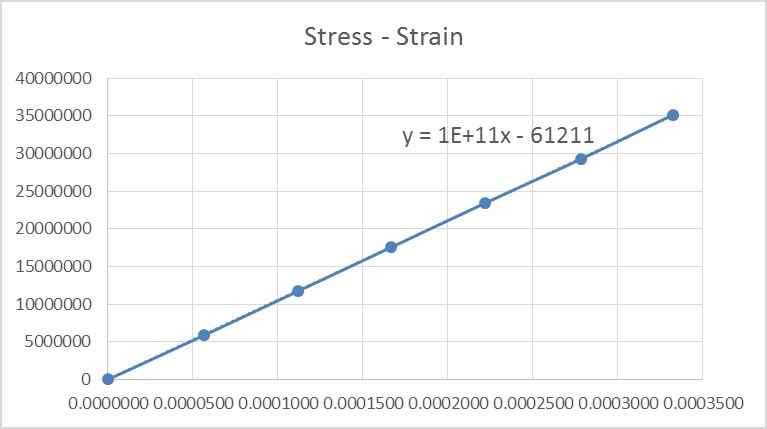
\includegraphics[width=0.7\linewidth]{8}
	\caption{Stress versus strain in Exp.4}
	\label{f8}
\end{figure}

\item
\textbf{Calculation of Young's modulus}\\
Due to the equation 
\begin{equation}
\sigma=Y\cdot \varepsilon
\end{equation}
Meanwhile, the linear relationship between stress and strain can be veried in graph. The slop of the line equation is Young's modulus. 

\begin{equation*}
\sigma=1.0\times 10^{11} \varepsilon-61211,\ where \ Y=1.0\times 10^{11} N/m^{2} 
\end{equation*}
Comparing the experimental value to the standard Young's modulus for brass, where$ Y=1.05\times 10^{11}$, the error is 

\begin{equation*}
Error=\frac{1.05-1.0}{1.05}\times 100\% \approx 4.76\%
\end{equation*}


\item 
\textbf{Comparison of strain on different position}\\

\begin{table}[!h]
	\centering
	\begin{tabular}{|c|c|c|c|c|}
		\hline
		\ &\multicolumn{2}{|c|}{Near the center} &\multicolumn{2}{|c|}{Near the pivots}\\
		\cline{2-5}
		Mass (kg) & $\delta V \ (mV)$ & $\ \varepsilon \ (10^{-3}) \ $ & $\delta V \ (mV)$& $\ \varepsilon \ (10^{-3}) \ $  \\
		\hline\hline
		0.0 & 0.048 & 0.000 &0.142 & 0.000\\
		\hline
		0.5 & 0.506 & 0.046 &0.318&0.032\\
		\hline
		1.0 & 0.060 & 0.102 &0.860 &0.085\\
		\hline
		1.5 & 0.580 & 0.157 &1.370 &0.136\\
		\hline
		2.0 & 2.110 & 0.214 &1.880 &0.186\\
		\hline
		2.5 & 2.620 & 0.269 &2.380 &0.236\\
		\hline
		3.0 & 3.130 & 0.325 &2.900 &0.287\\
		\hline
		
	\end{tabular}
	\caption{Comparison of strain on different position}
	\label{t5}
\end{table}

In order to compare the strain in two different position, calculate the values using $Equation\ (11)$. The results can be seen that, for same loading, the output voltage of gauges near the center is slightly larger than that near the pivots. Moreover, the strain values near the center is larger than that near the pivots. 
\end{enumerate}


\section{Experiment 5}
This experiment aims at investigating the modification to the stress pattern with a hole in the beam. The indicated picture is shown as below, and pairs of gauges are labeled as A and B. 

\begin{figure}[!h]
	\centering
	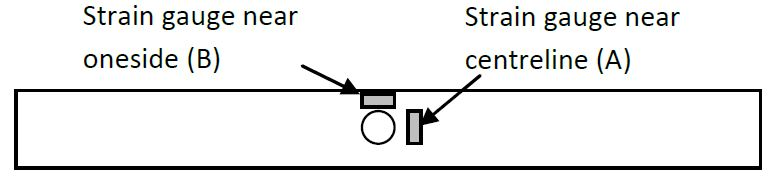
\includegraphics[width=0.6\linewidth]{9}
	\caption{Beam with a central hole}
	\label{f9}
\end{figure}

\subsection{Results}

\begin{table}[!h]
	\centering
	\begin{tabular}{|c||c|c|c|}
		\hline
		$Mass=3kg$ & $\delta V_{max} \ (mV)$ & $\ \varepsilon_{max} \ (10^{-3}) \ $ & $\sigma_{max} \ (10^{7})$ \\
		\hline\hline
		A & 1.53 & 0.302 &3.171 \\
		\hline
		B & 3.40 & 0.672 &7.055\\
		\hline
		Without Hole & 3.13 & 0.325 &3.413 \\
		\hline
	\end{tabular}
	\caption{Measurement and calaultion result of Exp.5}
	\label{t6}
\end{table}

\pagebreak

\subsection{Answsers to Questions}
\begin{enumerate}
\item
\textbf{Comparison of strains at position A and B} \\
Under the condition of same loading, the strain at B (with gauge near oneside) is larger than that at A (with gauge near centreline). The strain distribution on the beam is shown as below. According to the Mechanics of Materials and Elastic Mechanics, the strain line is along with the centreline and curve the edge of hole. Therefore, there is less strain on the centreline near the hole. \\

\begin{figure}[!h]
	\centering
	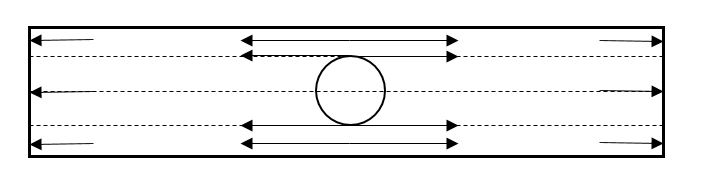
\includegraphics[width=0.6\linewidth]{10}
	\caption{Strain distribution on beam with a central hole}
	\label{f10}
\end{figure}

\item
\textbf{Comparison of strains under conditions with uniform beam} \\
As the Table\ref{t6} shows, comparing the first and last row, the strain on beam with a central hole is less than that at the uniform beam under same loading condition. Therefore, the exist of hole can disperse the strain near the centreline. However, the strain near oneside is larger than that at the uniform beam. \\

\item
\textbf{Calculation of stress concentration factor} \\
According to the formula 

\begin{equation}
K=\frac{\sigma_{max}(beam \ with\ hole)}{\sigma_{max}(beam \ without \ hole)}
\end{equation}

Therefore, for the slight different location at the center

\begin{equation*}
K\ =\frac{7.055}{3.171} \approx \textbf{2.225}
\end{equation*}


\item
\textbf{The effect of hole on stresses and strains} \\
From the view of Elastic Mechanics, the presence of the central hole has no effect on the stresses and strains at points remote from the hole. For the diameter of hole ($d=12mm$) is far smaller than the length of beam ($L=59cm$). Therefore, for the points far away from the hole, the distribution of strains and stresses is no difference. The hole disperse the strain and stress in the center, but concentrate the strain and stress around the hole evenly.  \\

\pagebreak

\section{Summary}
The strain gauge is an efficient tool to investigate the strains and stresses. Wheatstone bridge is used to detect the fractional change of resistance. When the object is deformed, the foil on gauge is deformed; thus its eletrical resistance changes. \\
In the first experiment, it is veried that the change output voltage is directly proport to the change of resistance.Therefore, we can just focus on the voltage change to analyze the strains. The use of another identical gauge to form the temperature compensation circuits lets the strain gauge changes only in response to applied strain. And the sensitivity of the strain can be doubled using multi-gauge bridge circuit.\\
With the Young's modulus as medium, the stress can be calculated with the value of strain. Experiment 4 shows that at the uniform beam, the stains at the center is larger than than near the pivots. However, the condition when a central hole is cut at the beam is complex. At the center, the strain is larger near the oneside than that near the centreline, but for the points far away from the hole, the consition is almost no difference. \\


\end{enumerate}
\end{document}